\documentclass[10pt,a4paper]{article}
\usepackage[margin=13mm]{geometry}
\usepackage{fontspec}
\IfFontExistsTF{Times New Roman}{\setmainfont{Times New Roman}}{\setmainfont{lmroman10-regular.otf}[BoldFont=lmroman10-bold.otf,ItalicFont=lmroman10-italic.otf,BoldItalicFont=lmroman10-bolditalic.otf]}
\IfFontExistsTF{Arial}{\setsansfont{Arial}}{\setsansfont{lmsans10-regular.otf}[BoldFont=lmsans10-bold.otf]}
\usepackage{graphicx,tabularx,array,enumitem,titlesec,xcolor}
\usepackage[colorlinks=true,urlcolor=blue!40!black,linkcolor=black]{hyperref}
\setlength{\parindent}{0pt}
\setlength{\parskip}{2pt}
\setlength{\tabcolsep}{0pt}
\pagestyle{empty}
\titleformat{\section}{\large\sffamily\bfseries}{}{0pt}{}[\titlerule]
\titlespacing*{\section}{0pt}{7pt}{4pt}
\newcommand{\entry}[3]{\noindent\begin{tabularx}{\textwidth}{@{}p{32mm}@{\hspace{3mm}}X@{}}{\small\raggedright #1} & \begin{minipage}[t]{\linewidth}\raggedright\textbf{#2}\par #3\end{minipage}\end{tabularx}\par\vspace{3pt}}
\newcommand{\paper}[4]{\entry{#1}{#2}{#3\\#4}}
\newcommand{\links}[1]{{\small #1}}
\begin{document}
\begin{minipage}[c]{0.83\textwidth}
{\Huge\sffamily\bfseries Zhu Yufan}\\[4pt]
\href{mailto:yufan.zhu@u.nus.edu}{yufan.zhu@u.nus.edu}\quad
\href{mailto:zhuyf@a-star.edu.sg}{zhuyf@a-star.edu.sg}\\[2pt]
\href{https://yufannnn.github.io/}{Personal website}\quad
\href{https://scholar.google.com/citations?user=zbe0xWAAAAAJ}{Google Scholar}\quad
\href{https://github.com/Yufannnn}{GitHub}\quad
\href{https://huggingface.co/HenryZYF}{Hugging Face}\quad
\href{https://www.linkedin.com/in/yufan-zhu-36024a225/}{LinkedIn}
\end{minipage}\hfill
\begin{minipage}[c]{0.13\textwidth}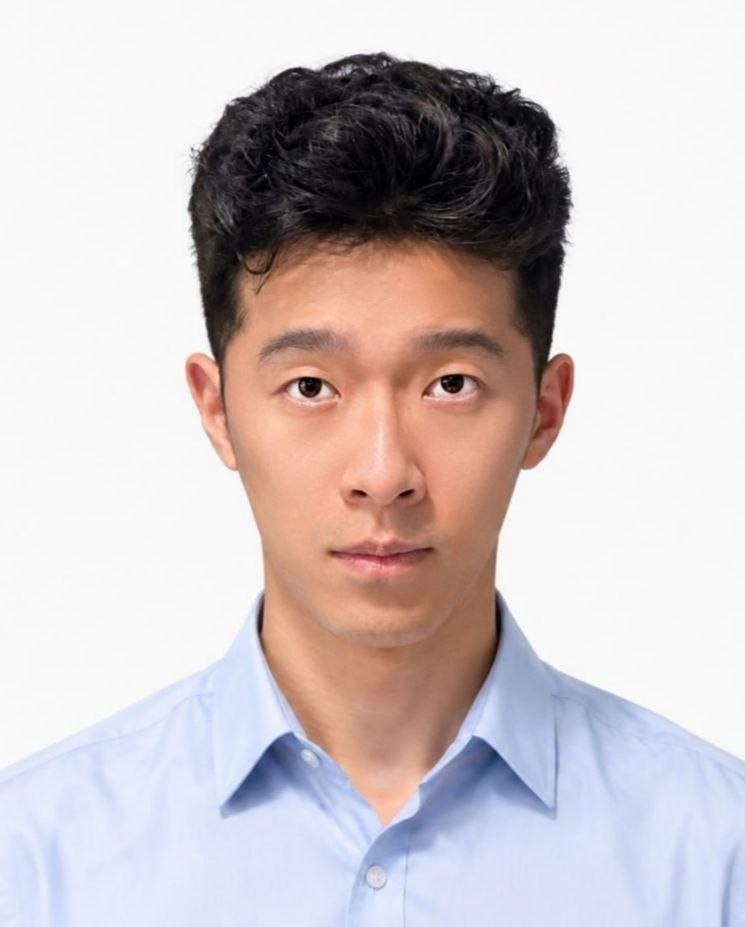
\includegraphics[width=\linewidth]{photo.jpg}\end{minipage}

\section*{RESEARCH INTERESTS}
Large Language Models; Natural Language Processing; Data Privacy and Sanitization;\\
Privacy-Preserving Machine Learning; Applied Cryptography.

\section*{EDUCATION}
\entry{Aug 2025 -- May 2029}{National University of Singapore}{Ph.D. in Computer Science. Research focus: LLM security, data privacy, and privacy-preserving machine learning.}
\entry{Aug 2021 -- May 2025}{National University of Singapore}{B.Comp. in Computer Science, Second Major in Statistics (Highest Distinction).\\GPA: 4.6/5.0. Focus areas: Artificial Intelligence and Databases.}
\entry{Feb 2019 -- Dec 2020}{Eunoia Junior College}{A Level result: AAAA/A.}

\section*{SCHOLARSHIPS AND AWARDS}
\begin{tabularx}{\textwidth}{@{}p{30mm}@{\hspace{3mm}}X@{}}
2025--2029 & NUS Research Scholarship Recipient\\
2021--2025 & NUS Science and Technology Merit Scholarship Recipient\\
2016--2020 & MOE School-based Scholarship (SM1 Scholarship) Recipient
\end{tabularx}

\section*{RESEARCH PUBLICATIONS AND MANUSCRIPTS}
\paper{2026}{QuasiLeak-Bench: Evaluating LLM-Based Privacy Detectors on Policy-Conditioned Quasi-Evidence Group Recovery}{\textbf{Yufan Zhu}, Yangfan Jiang, Yang Fei, Shizheng Hou, Shubhankar Mohapatra, Xiaokui Xiao.}{\emph{ARR submission.}\\\links{\href{https://arxiv.org/abs/2610.21333}{arXiv}\quad\href{https://arxiv.org/pdf/2610.21333}{PDF}\quad\href{https://github.com/Yufannnn/QuasiLeak-Bench}{Code}\quad\href{https://huggingface.co/datasets/HenryZYF/QuasiLeak-Bench}{Dataset}\quad\href{https://yufannnn.github.io/QuasiLeak-Bench/}{Leaderboard}}}
\paper{2026}{FESC: Remodeling Long-Context Private Inference with Encrypted State-Space Models}{\textbf{Yufan Zhu}, Chao Jin, Khin Mi Mi Aung, Xiaokui Xiao.}{\emph{NDSS submission (NDSS 2027).}\\\links{\href{https://arxiv.org/abs/2608.17442}{arXiv}\quad\href{https://arxiv.org/pdf/2608.17442}{PDF}\quad\href{https://github.com/Yufannnn/FESC}{Code}}}
\paper{2026}{EncFormer: Secure and Efficient Transformer Inference over Encrypted Data}{\textbf{Yufan Zhu}, Chao Jin, Khin Mi Mi Aung, Xiaokui Xiao.}{\emph{IEEE Transactions on Dependable and Secure Computing (TDSC). Accepted for publication.}\\\links{\href{https://arxiv.org/abs/2604.09975}{arXiv}\quad\href{https://arxiv.org/pdf/2604.09975}{PDF}\quad\href{https://github.com/Yufannnn/EncFormer}{Code}\quad\href{https://yufannnn.github.io/EncFormer/}{Demo}}}
\paper{2024}{A Personalized Learning Tool for Physics Undergraduate Students Built on a Large Language Model for Symbolic Regression}{\textbf{Yufan Zhu}, Zi-Yu Khoo, Jonathan Sze Choong Low, St\'ephane Bressan.}{\emph{Proceedings of the 2024 IEEE Conference on Artificial Intelligence.}\\\links{\href{https://ieeexplore.ieee.org/document/10605241}{Publisher}\quad\href{https://ieeexplore.ieee.org/stamp/stamp.jsp?tp=\&arnumber=10605241}{PDF}}}

\section*{PROFESSIONAL SERVICE}
\entry{2026}{Reviewer}{ACM International Conference on Information and Knowledge Management (CIKM 2026).\\IEEE Transactions on Information Forensics and Security (TIFS).}

\section*{RESEARCH EXPERIENCE}
\entry{Aug 2024 -- Present}{Graduate Research Assistant, National University of Singapore \& A*STAR}{Developing LLM privacy evaluation and privacy-preserving inference systems with Professor Xiaokui Xiao and Dr. Chao Jin, including QuasiLeak-Bench, FESC, and EncFormer.}
\entry{Jul 2024 -- Jan 2025}{Research Assistant, Nanyang Technological University, Centre for Quantum Technologies \& A*STAR}{Co-developed an autonomous quantum agent using variational quantum algorithms for memory-efficient data stream classification with Professor Mile Gu and Dr. Jayne Thompson, outperforming classical RNN baselines.}
\entry{May 2024 -- Aug 2024}{Research Assistant (Odyssey), National University of Singapore}{Built a theory-driven AIGC framework for visual marketing with Ph.D. candidate Bruce Yang under Professors Xiaofan Li and Dandan Qiao, evaluating creativity and effectiveness against professionally generated content.}

\section*{EMPLOYMENT HISTORY}
\entry{May 2024 -- Aug 2024}{Machine Learning Research Engineer Intern, A*STAR}{Conducted model training and compatibility validation for machine learning on encrypted data. Developed testing frameworks for software and API layers, with a focus on model optimization and data security.}
\entry{May 2023 -- Aug 2023}{Generative Artificial Intelligence Engineer Intern, KiWi Augmented Retail Technology}{Led a three-person team in building an automated poster-generation pipeline using Stable Diffusion and LLMs. Oversaw the product roadmap, backend API architecture, microservices deployment, and object-recognition capabilities.}

\section*{TEACHING AND RELATED EXPERIENCE}
\entry{Aug 2022 -- May 2025}{Teaching Assistant, National University of Singapore}{Conducted tutorials and labs, graded assignments, held consultations, supervised student projects, and structured exam questions for CS1101S (Programming Methodology), CS2100 (Computer Organization), CS2106 (Introduction to Operating Systems), and CS4248 (Natural Language Processing).}
\entry{Nov 2022 -- Present}{Student Tutor, Raffles Institution Boarding School}{Mentor and tutor boarders, lead house events, and liaise with staff and parents on student welfare.}

\section*{PROJECT EXPERIENCE}
\entry{2026}{QuasiLeak-Bench --- LLM Privacy Evaluation}{Built a benchmark for policy-conditioned quasi-evidence group recovery, with 5,000 documents, 500 profiles, a released scorer and dataset, and an interactive leaderboard. ARR submission.}
\entry{2026}{FESC --- Private Long-Context Inference}{Developed a hybrid encrypted inference system for selective state-space models, using a factorized scan-contract and GPU-optimized linear kernels. NDSS submission.}
\entry{2024}{SplaXBERT for Question Answering (CS4248)}{Led a four-person team in fine-tuning an enhanced BERT-based model for SQuAD v1.1, balancing model complexity and question-answering accuracy.}
\entry{2023}{Bayesian Stroke Prediction (CS3263)}{Led a three-person team in developing a Bayesian stroke-prediction model; received the Best Project Award under Professor Tze Yun Leong.}
\entry{2023}{TutorPro (CS2103T)}{Led a four-person team in creating a desktop application to simplify private tutors' administrative workflows.}
\entry{2022}{AI Agent for Breakthrough (CS2109S)}{Designed a board-game agent using iterative-deepening minimax search.}

\section*{VOLUNTEER EXPERIENCE}
\entry{Aug 2019}{Programming Mentor for Underprivileged Children}{Taught Scratch to primary-school students from low-income families.}
\end{document}
